The inference part contains the 4 following functionalities:

\begin{itemize}[label=(\roman*)]
\item \mintinline{python}{romc.sample(n2, seed=None)}
\item \mintinline{python}{romc.compute_expectation(h)}  
\item \mintinline{python}{romc.eval_unnorm_posterior(theta)}
\item \mintinline{python}{romc.eval_posterior(theta)}
\end{itemize}

\subsubsection*{Function (i): Perform weithted sampling}

\mintinline{python}{romc.sample(n2)}
\vspace{5mm}

\noindent
This is the basic inference utility of the ROMC implementation; we
draw $n_2$ samples for each bounding box region. This gives a total of
$k \times n_2$, where $k < n_1$ is the number of the optimal points
remained after filtering\footnote{From the $n_1$ optimisation
  problems, only the ones with $g_i(\thetab_*) < \epsilon$ are kept
  for building a bounding box}. The samples are drawn from a uniform
distribution $q_i$ defined over the corresponding bounding box and the
weight $w_i$ is computed as in equation~\eqref{eq:sampling}. The
function stores an \pinline{elfi.Result} object as
\pinline{romc.result} attribute. The \pinline{elfi.Result} provides
some usefull functionalities for inspecting the obtained samples e.g.\
\pinline{romc.result.summary()} prints the number of the obtained
samples and their mean. A comlete overview of these functionalities is
provided in ELFI's
\href{https://elfi.readthedocs.io/en/latest/api.html#elfi.methods.results.Sample}{official
  documentation}.

\subsubsection*{Function (ii): Compute an expectation}

\mintinline{python}{romc.compute_expectation(h)}
\vspace{5mm}

\noindent
This function computes the expectation
$E_{p(\thetab|\data)}[h(\thetab)]$ using
expression~\eqref{eq:expectation}. The argument \pinline{h} can be
any python \pinline{Callable}.

\subsubsection*{Function (iii): Evaluate the unnormalised posterior}
\mintinline{python}{romc.eval_unorm_posterior(theta, eps_cutoff=False)}
\vspace{5mm}

\noindent
This function computes the unnormalised posterior approximation using
expression~\eqref{eq:approx_posterior}.

\subsubsection*{Function (iv): Evaluate the normalised posterior}
\mintinline{python}{romc.eval_posterior(theta, eps_cutoff=False)}
\vspace{5mm}

\noindent
This function evaluates the normalised posterior. For doing so it
needs to approximate the partition function
$Z = \int p_{d,\epsilon}(\thetab|\data)d\thetab$; this is done using
the Riemann integral aproximation. Unfortunatelly, the Riemann
approximation does not scale well in high-dimensional spaces, hence
the approximation is tractable only at low-dimensional parametric
spaces. Given that this functionality is particulary useful for
ploting the posterior, we could say that it is meaningful to be used
for up to $3D$ parametric spaces, even though it is not restricted to
that. Finally, for this functionality to work, the \pinline{bounds}
arguments must have been set at the initialisation of the
\pinline{elfi.ROMC} object.\footnote{The argument \pinline{bounds}
  should define a bounding box \emph{containing} all the mass of the
  prior; it may also contain redundant areas. For example, if the
  prior is the uniform defined over a unit circle i.e.\
  $c=(0,0), r=1$, the best bounds arguments is
  \pinline{bounds=[(-1,1),(-1,1)]}. However, any argument
  \pinline{bounds=[(-t,t),(-t,t)]} where $t\geq1$ is technically
  correct.}

\subsubsection*{Example - Sampling and compute expectation}

With the following code snippet, we perform weighted sampling from the
ROMC approximate posterior. Afterwards, we used some ELFI's built-in
tools to get a summary of the obtained samples. In figure
\ref{fig:example_sampling}, we observe the histogram of the weighted
samples and the acceptance region of the first deterministic function
(as before) alongside with the obtained samples obtained from
it. Finally, in the code snippet we demonstrate how to use the
\pinline{compute_expectation} function; in the current example we
define \pinline{h} in order to compute firstly the empirical mean and
afterwards the empirical variance. In both cases, the empirical result
is close to the ground truth $\mu = 0$ and $\sigma^2 = 1$.

\begin{pythoncode}
  seed = 21
  n2 = 50
  romc.sample(n2=n2, seed=seed)

  # visualize region, adding the samples now
  romc.visualize_region(i=1)

  # Visualise marginal (built-in ELFI tool)
  romc.result.plot_marginals(weights=romc.result.weights, bins=100, range=(-3,3))

  # Summarize the samples (built-in ELFI tool)
  romc.result.summary()
  # Number of samples: 1720
  # Sample means: theta: -0.0792

  # compute expectation
  print("Expected value   : %.3f" % romc.compute_expectation(h=lambda x: np.squeeze(x)))
  # Expected value   : -0.079

  print("Expected variance: %.3f" % romc.compute_expectation(h=lambda x: np.squeeze(x)**2))
  # Expected variance: 1.061
\end{pythoncode}

\begin{figure}[h]
    \begin{center}
      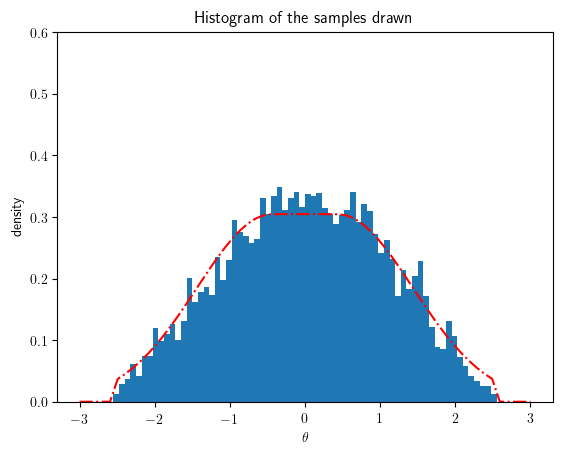
\includegraphics[width=0.48\textwidth]{./Thesis/images/chapter3/example_marginal.png}
      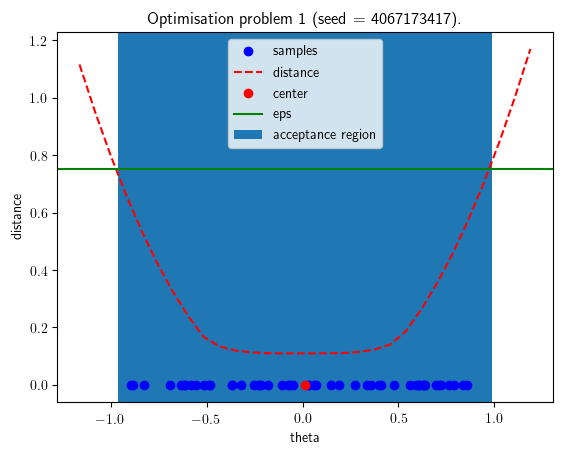
\includegraphics[width=0.48\textwidth]{./Thesis/images/chapter3/example_region_samples.png}
    \end{center}
  \caption[Histogram of the obtained samples at the 1D example.]{(a) Left: Histogram of the obtained samples. (b) Right: Acceptance region around $\theta_1^*$ with the obtained samples plotted inside.}
  \label{fig:example_sampling}
\end{figure}

\subsubsection*{Example - Evaluate Posterior}

The \pinline{romc.eval_unnorm_posterior(theta)} evaluates the
posterior at point $\theta$ using expression
\eqref{eq:aprox_posterior}. The \pinline{romc.eval_posterior(theta)}
approximates the partition function
$Z = \int_{\thetab} p_{d,\epsilon}(\thetab|\data) d\thetab$ using the
Riemann approximation as explained above. In our simple example, this
utility can provide a nice plot of the approximate posterior as
illustrated in figure~\ref{fig:approx_posterior}. We observe that the
approximation is quite close to the ground-truth posterior.

\begin{figure}[ht]
    \begin{center}
      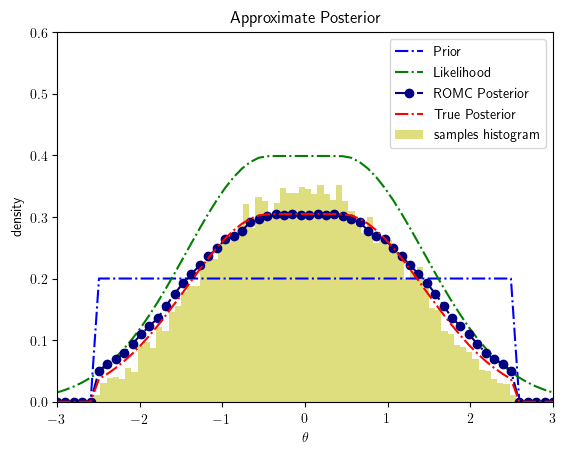
\includegraphics[width=0.75\textwidth]{./Thesis/images/chapter3/example_posterior.png}
    \end{center}
  \caption[Approximate posterior evaluation, at the 1D example.]{Approximate posterior evaluation.}
  \label{fig:approx_posterior}
\end{figure}
